\chapter{Tools and their artefacts}~\label{chapter-tools-and-their-artefacts}
%\julian{This chapter covers \utools and \itools.}

This chapter covers two of the six perspectives, \emph{i.e.} using and improving mobile analytics tools. The primary evidence comes from both the app-centric and the tools-centric case studies, augmented with material from grey data and grey literature.

The evidence has been analysed and prioritised to keep the chapter relatively succinct and on topic. 38 L1 themes emerged in the analysis of the evidence, of these the ones with strongest support in terms of the evidence are included here, the rest would benefit from further work.

The top ranked L1 themes are core to this chapter and they are: 
{\small
\begin{enumerate}
    \itemsep0em
    \item[1] sdk-design: the design of the client-side SDK affects many aspects of the data collection which then feeds subsequent stages in the processing of the data to provide the mobile analytics.
    \item[1] ux-design: The design of the User Experience (UX) of the mobile analytics tool for their audience of the software development team (and particularly the app developers).
    \item[3] product-fit: whether, and if practical how well, the mobile analytics product fits the desires/needs of the developers. 
    \item[4] actionable-reports: reports the developers can action in order to address concerns presented in the reports.    
    \item[4] integration-into-workflows: the ability of a given mobile analytics tool/service to be integrated into development team's workflows.
    \item[6] meta-data: data not directly about the app, instead it's data about the user and/or their device, etc.
    \item[7] flaws: weaknesses, mistakes, errors, etc. pertaining to the mobile analytics tool/service.
    \item[8] ethical-considerations: the data collected by mobile analytics may have ethical implications a) for the operator/provider of the service, b) for their partners and customers, c) for the developers, d) for end-users. In this research our main focus is on the implications for the developers, nonetheless the other aspects are also important.
    \item[8] link-rot-preservation-of-results: the validity of a URL may be finite, as may the contents be even if the link remains. For mobile analytics services link rot is often a common reason why results are no longer available from the mobile analytics service - the link was ephermeral. In such cases the results would need to be preserved while the results are still available. In some cases the rot may be easy to predict, for instance as data ages beyond the predefined date range of a report, in other cases less so, for instance when the active release is updated the data for the previous currently active release might 'disappear' from some reports.
    \item[10] benefits-of-combining-mobile-analytics-tools: an observation of benefits developers can obtain through combining their use of several mobile analytics tools.
    \item[11] bug-localisation: features in the tool that may enable developers to localise one or more bugs.
    \item[12] efficacy-of-tool: how efficient and how effective is the tool, i.e. how efficacious is the tool? Did it achieve the objectives it claims to achieve?
    \item[12] engineering-challenges: Engineering challenges related to developing the components of the mobile analytics tool/service such as provision of a client-side SDK that collects failures for native (C++) code.
    \item[12] return-on-investment: developers may make both implicit and explicit choices on what to invest in, for instance in terms of their focus, their effort, and their money. The analytics tools need to convince developers a) to invest and then b) whether to increase that investment (and if so what forms of investment e.g. in terms of writing more code, spending [more] money, using the tool more, etc.).
    \item[12] testability: the ability to test the overall service, the tool, and/or components that comprise the analytics tool.
    \item[12] vying-for-attention-of-developers: mobile analytics competes (vies) for the attention of the app developers against a plethora of other competing demands, offerings, and constraints. 
\end{enumerate}
}

These can be aggregated into four higher-level (L2) themes: design, fit-for-purpose, utility, dependability. Figure \ref{fig:analytics-tools-and-their-artefacts-fishbone-diagram} illustrates the top L1 themes and their main higher-level (L2) theme.

\begin{figure}
    \centering
    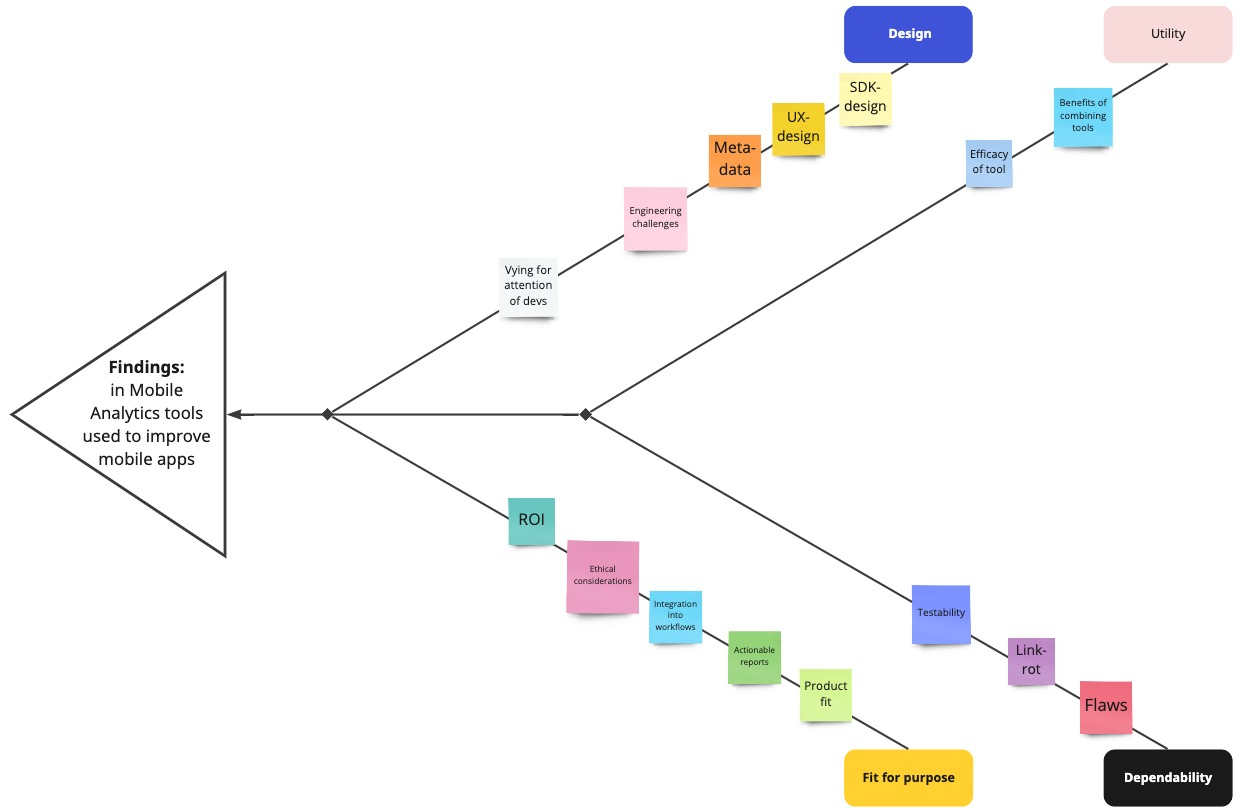
\includegraphics[width=\textwidth]{images/rough-sketches/analytics-tools-and-their-artefacts-fishbone-diagram-14-jun-2022a.jpeg}
    \caption{Analytics Tools and their Artefacts Fishbone Diagram\\Source: \href{https://miro.com/app/board/uXjVOtIsyWo=/?share_link_id=293061080490}{Miro}}
    \label{fig:analytics-tools-and-their-artefacts-fishbone-diagram}
\end{figure}

\section{Design}
Design of the SDK and the developer-experience (UX) of the mobile analytics emerged as the top two ranked themes for analytics tools. Any in-app SDK needs to integrate easily in to the mobile app and platform-level analytics needs to be seamless and collect sufficient pertinent information to be useful for the app developers. They also need to be robust and timely in terms of collection, transmission, and processing of the underlying data in order for developers to have timely access to the results. 

Fabric Crashlytics is the archetypal example of how a mobile analytics tool can be designed to serve developers well. The product team developed it from the ground up, starting with excellent crash reporting, to provide developers with timely, actionable, attractive, and useful reports. This led to it becoming one of the top three mobile analytics tools for both iOS and Android within 10 months of being launched~\citep{___answersblog_2015_may_crashlytics-no1-in-performance}. % See also https://web.archive.org/web/20151203150947/http://fabric.io/blog/crashlytics-answers-named-top-mobile-sdks
First Twitter acquired it and then Google did; they subsequently integrated it into Firebase Analytics which is the most popular mobile analytics service for Android apps currently.

Platform-level analytics provides an outsider's perspective on the behaviour of mobile app, in contrast to in-app analytics that provides an insider's perspective. In this research Google's Android Vitals provides the platform-level analytics as it has the largest reach of any platform-level analytics across the widest range of devices. The platform provides users the ability to allow or deny analytics to be sent from their device. Apple's iOS (and MacOS) ask the user explicitly~\citep{apple_ios_share_diagnostics}, Android does not - users need to find the setting and opt-out~\citep{google_play_share_usage_and_diagnostics_info_with_google}. % See also https://chefkochblog.wordpress.com/2018/02/09/how-to-disable-android-usage-diagnostics-sharing/ I've not referenced this as they don't provide evidence of the default settings.

Mobile Analytics tools vie for attention against a plethora of other developer-oriented tools, project demands, \emph{etc.} Developers need to be enticed into using the tools and then retained on an ongoing basis to meet the objectives of the providers of the mobile analytics services.

\subsection{SDK design}
Any mobile analytics SDK needs to be designed to collected relevant data and forward that data so it can be processed, analysed, and reported on. 

\textbf{Programming language support}: 
Mobile apps %are written using hybrid/cross platform-frameworks, others in platform/managed code, a few may be written purely in native/unmanaged code, and some combine several of these. They 
can be written in several programming languages. While many mobile apps are written in a single programming language some use several programming languages, for instance Kiwix Android combines Java, Kotlin, and C++. 
% More reading on Cordova's demise: https://medium.com/codex/the-sunset-of-apache-cordova-alternatives-for-cross-platform-mobile-development-in-2022-9da34234c992

Mobile analytics SDKs, in turn, support one or more of the programming languages. If they do not support the programming languages then they may not be able to obtain or provide analytics for elements written in the unsupported programming languages. For C and C++ code in particular, the app developers generally need to explicitly configure the code and the build process to incorporate the relevant mobile analytics SDK if it's available. % For a counterexample Fabric Crashlytics claimed their SDK was very easy to integrate https://web.archive.org/web/20151019132428/https://crashlytics.com/blog/the-wait-is-over-launching-crashlytics-for-android-ndk

\textbf{SDK initialisation}: 
The SDK needs to be initialised as early as practical each time the app is started (or restarted) if it's to capture pertinent information (including crashes that occur when the app starts or restarts). For mobile analytics SDKs this has led to their developers finding and implementing mechanisms to initialise their SDK in innovative (and unusual) ways, for instance Firebase uses a ContentProvider~\citep{stevenson2016_how_does_firebase_initialize_on_android}. Note: this does not always work, as reported in \citep{reddy2022_crashlytics_fails_to_track_app_startup_crashes}. When the SDK initialises it obtains various meta data about the app and the device. 

\textbf{Meta-data}: 
Figure \ref{fig:fabric-crashlytics-privacy-policy} provides an illustration of the privacy policy for Fabric Crashlytics which lists various the meta-data it collected at the time. The successor Firebase Crashlytics lists similar data being collected for crashes~\url{https://firebase.google.com/support/privacy#crash-stored-info}. The details of why these details were necessary was discussed online~\citep{kim2017_what_information_does_crashlytics_collect_from_end_users}.

\begin{figure}
    \centering
    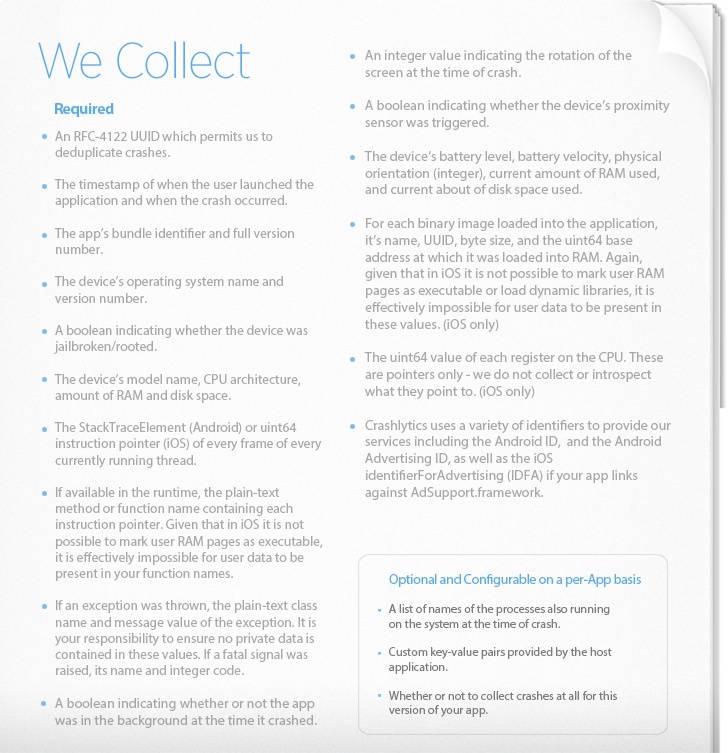
\includegraphics[width=10cm]{images/fabric-crashlytics/crashlytics-privacy-policy-38154ffbd69ef44a478b54365dc9b3ad.png}
    \caption{Fabric Crashlytics Privacy Policy (in 2015)\\{source: \tiny \url{https://web.archive.org/web/20150405071731/http://try.crashlytics.com/security/}}}
    \label{fig:fabric-crashlytics-privacy-policy}
\end{figure}

However, some app developers may receive data they didn't expect, particularly if they migrated from Fabric Crashlytics to Firebase Crashlytics. 

To provide some additional context Fabric and Firebase both offered facilities to combine various datasets into their reporting, for instance based on advertising SDKs. This led to reports that include demographics in addition to the crash analytics, \emph{etc.}~\footnote{Discussions on how the demographics are captured and made available include~\citep{joe2016_firebase_analytics_demographics} and~\citep{chelo2020_firebase_does_not_collect_age_or_gender_data}.}. 

The forced migration from Fabric Crashlytics to Firebase Crashlytics had two stages, the first was to migrate the project to the Firebase user interface and the second was to replace the Fabric SDK with the Firebase SDK. The Firebase SDK automatically collected additional data~\citep{firebase_help_GA4_2021_predefined_user_dimensions}.

As mentioned in the previous chapter, the Catrobat project chose to stop using Firebase Crashlytics when they discovered the demographics of the end users was also being recorded. 
%

In collaborative research into using Firebase Analytics for logging, 50 of 107 active Android opensource projects initialised just the Firebase Analytics SDK, they did not use any other aspect of the SDK~\citep{harty2021_logging_practices_with_mobile_analytics}~\footnote{Perhaps they thought that `Getting Started' was all they needed to do? or perhaps the default data was `good enough'?}. Therefore the contents and the limitations of the default meta-data are of particular interest since it is all those developers would have available to them. The remaining 57 projects used additional API calls to record additional information on one or more code-paths in the respective app.

\textbf{Runtime activities for the SDK}: 
When the SDK is running, which they do in the background without being visible to the user of the app, they are responsible for the safekeeping and transmission of the collected data. Some collect data automatically, or autonomously. For example, Sentry's in-app SDK collects `automatic instrumentation'~\citep{sentry2021_mobile_vitals_four_metrics_every_mobile_developer_should_care_about}, and Android Vitals collects usage data, app crashes, and ANRs automatically.

At least some of the SDKs store analytics data locally on the device on an interim basis, the stored data would be removed once it had been successfully transmitted. Various SDKs limit the number of items they store. The SDKs also vary in how and when they transmit the data and on their behaviour if there isn't a suitable network connection to transmit the data.

\textbf{Limitations in visibility by an SDK}: 
In short, the viewpoint of the SDK affects and can limit what it can observe/record. Also some mobile apps incorporate their own runtime which may hide some failures from being observed by the platform.

\textbf{Android Vitals}: 
Android Vitals does not collect crashes that are contained within an application's runtime. React-Native is a popular cross-platform app development framework. It includes its own application runtime environment and this runtime automatically restarts the app if it crashes. These crashes are not visible to Android Vitals as evidenced by two of the apps within the app centric case studies: LocalHalo and Taskinator where Android Vitals showed no crashes for either these apps, with one exception. 

\textbf{Some failures did emerge}:
That exception was when Android Vitals did report crashes in March and April 2020. Figure \ref{fig:localhalo-android-vitals-no-data-16-march-2020} was recorded on \nth{16} March 2020 before these started and shows the App Health Overview page with a link to a video introducing Android Vitals~\footnote{This appears as a mainly black rectangle in this thumbnail screenshot.}, and the App Health Details page with no data.

\textbf{In-app analytics support for detecting ANRs}: 
Conversely, in-app analytics SDKs were not able to measure ANRs which meant Android Vitals was the primary source of ANR analytics for Android app developers~\footnote{There is an opensource utility that uses a watchdog timer to detect ANRs~\citep{salomonbrys_github_anr_watchdog}. Investigating it was beyond the scope of the immediate research, nonetheless Sentry used that code as a basis for their ANR reporting (\href{https://github.com/getsentry/sentry-java/blob/3f8d7b1cc869bb056c9db99b459e43f6c375784a/sentry-android-core/src/main/java/io/sentry/android/core/ANRWatchDog.java}{sentry-android-core...ANRWatchDog.java}).}. 

Note: Google has subsequently added a mechanism to enable apps to obtain information about previous ANRs when the app next started. The method is \href{https://developer.android.com/reference/kotlin/android/app/ActivityManager#gethistoricalprocessexitreasons}{\texttt{getHistoricalProcessExitReasons()}}~\footnote{The source code is available online: \url{https://android.googlesource.com/platform/frameworks/base/+/master/core/java/android/app/ApplicationExitInfo.java} and provides more details of the design and the data structures.}, added in \href{https://developer.android.com/about/versions/11}{Android 11}, API level 30.
% Various discussions and explanations of using this API follow:
% https://commonsware.com/R/pages/chap-dataaccess-002.html - possibly the best and clearest code examples with explanations.
% Announcing the new functionality in 2021 https://firebase.blog/posts/2021/11/whats-new-at-Firebase-Summit-2021
% https://medium.com/@yangweigbh/monitoring-app-termination-on-android-11-97d514a3f9 
% Facebook's SDK to obtain cached ANRs https://developers.facebook.com/docs/reference/androidsdk/current/facebook/com/facebook/internal/instrument/anrreport/anrhandler.html/ and https://github.com/facebook/facebook-android-sdk/blob/5fe6e2a9d7056a17f54c1cae13e00788723d34f6/facebook-core/src/main/java/com/facebook/internal/instrument/anrreport/ANRHandler.kt
%
At the time of writing, Firebase Analytics uses this mechanism to obtain the ANR and other app exit data, see \href{https://github.com/firebase/firebase-android-sdk/blob/73131b69b0134456441e7fa218964b6a766fcec7/firebase-crashlytics/src/main/java/com/google/firebase/crashlytics/FirebaseCrashlytics.java}{\texttt{github.com.........FirebaseCrashlytics.java}}.

\subsection{LocalHalo React Native example}
The LocalHalo app-centric case study provides an illustration where app crashes were not observed by Android Vitals until a failure in the React Native runtime occurred.

\begin{figure}[htbp!]
\centering
\begin{minipage}{.45\textwidth}
  \centering
  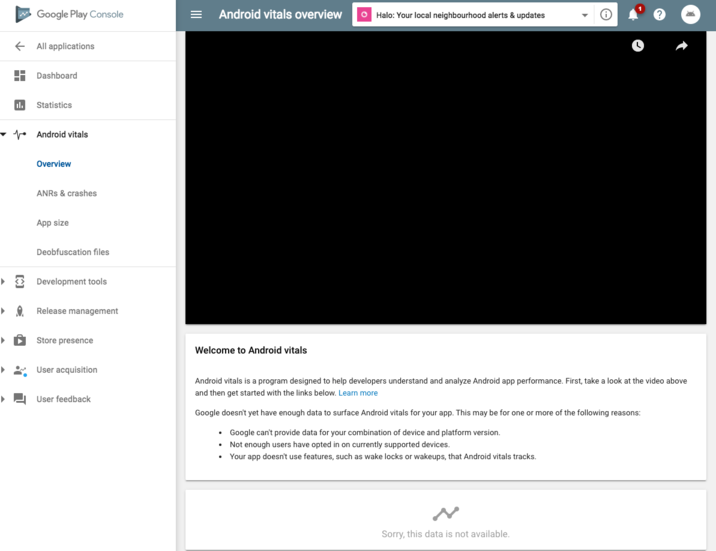
\includegraphics[width=\textwidth]{images/localhalo/apphealthoverviewplace_5550596_no_data.png}
  \captionof*{figure}{App Health Overview page}
\end{minipage}\hfill%
\begin{minipage}{.45\textwidth}
  \centering
  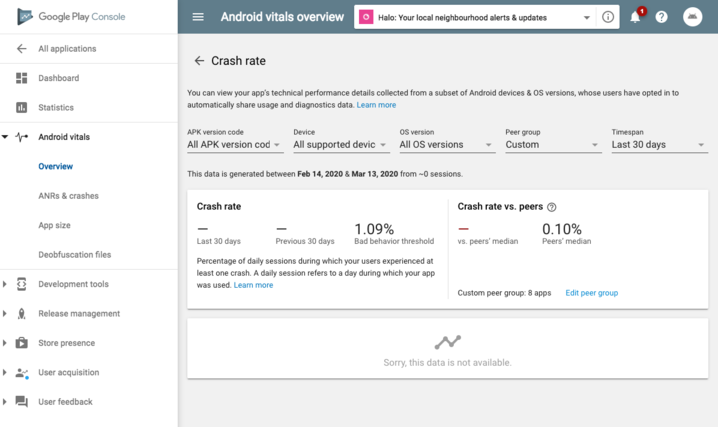
\includegraphics[width=\textwidth]{images/localhalo/apphealthdetailsplace_55505963_no_data.png}
  \captionof*{figure}{App Health Details page}
\end{minipage}
    \caption{No Android Vitals reports on \nth{16} March 2020}
    \label{fig:localhalo-android-vitals-no-data-16-march-2020}
\end{figure}

Figure~\ref{fig:localhalo-android-vitals-high-failures-26-march-2020} was recorded ten days later in \nth{26} March 2020 and shows the alerts for both high crash and ANR rates in the App Health Overview page and the graph for the rampant crash rate in the corresponding App Health Details page. These indicate the failures were related to the native runtime rather than within the React Native code. These were not reported by any Sentry Alerts and they do not appear in the weekly summary reports, except potentially by the absence of data shown in Figure~\ref{fig:sentry-missing-data-march-2020}. While the reason for this was not explained in the interviews or in the analytics data, it is likely that this caused by severe crashes that prevented Sentry's SDK from reporting any data.

\begin{figure}[htbp!]
\centering
\begin{minipage}{.45\textwidth}
  \centering
  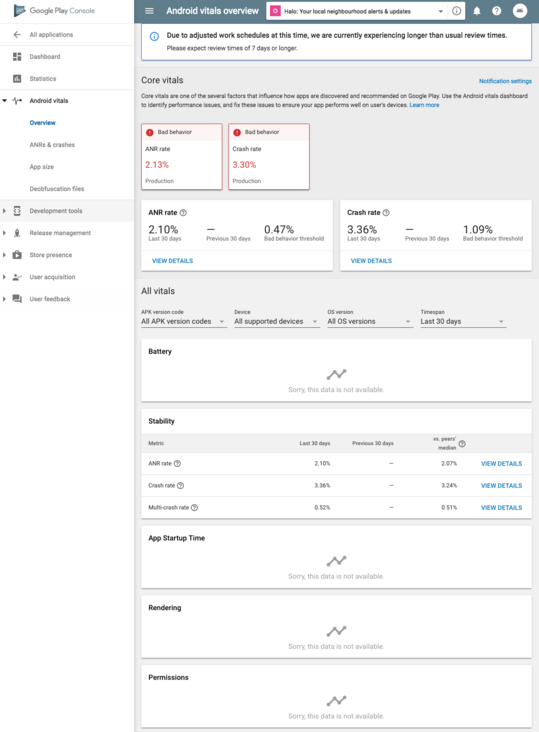
\includegraphics[width=\textwidth]{images/localhalo/apphealthoverviewplace_5550596_high_errors.png}
  \captionof*{figure}{App Health Overview page}
\end{minipage}\hfill%
\begin{minipage}{.45\textwidth}
  \centering
  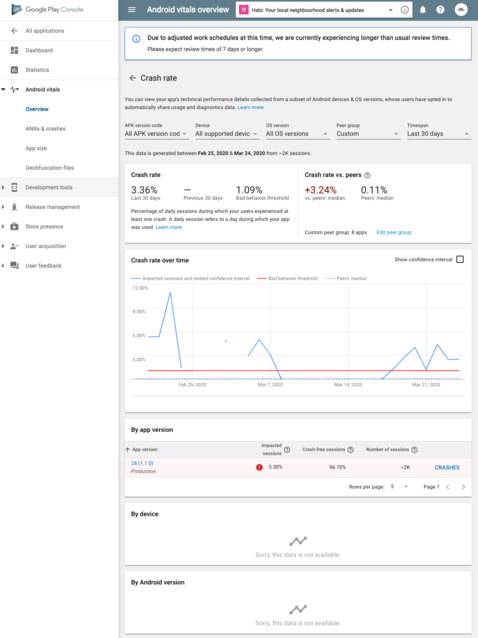
\includegraphics[width=\textwidth]{images/localhalo/apphealthdetailsplace_55505963_high_errors.png}
  \captionof*{figure}{App Health Details page}
\end{minipage}
    \caption{Alerts and graphs in Android Vitals on \nth{26} March 2020}
    \label{fig:localhalo-android-vitals-high-failures-26-march-2020}
\end{figure}

A release in March 2020 had a high crash rate for the production release of their Android app. The top crash cluster was for:

{\small \texttt{java.lang.RuntimeExceptionhost.exp.exponent.experience.a\$b.run}} 

This was traced to a problem in the expo library the development team used in the app~\citep{expo2019_issue5839}~\footnote{Expo is a very popular opensource platform for making universal native apps that run on Android, iOS, and the web \url{https://github.com/expo/expo}.}. In that issue several developers for different Android apps provide data from Google Play Console confirming they also receive similar crash clusters. The cause has not yet been definitively traced or addressed, however for the LocalHalo app the crashes stopped being reported once a new release of the Android app, release 1.3.0, was released around \nth{6} April 2020.


\begin{figure}[htbp!]
\centering
\begin{minipage}{.45\textwidth}
  \centering
  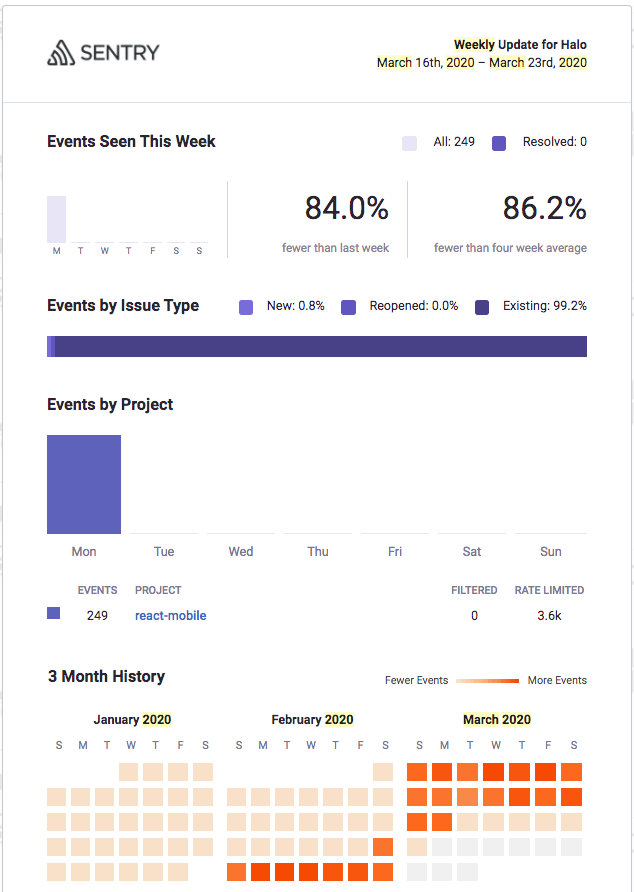
\includegraphics[width=\textwidth]{images/localhalo/sentry-weekly-report-16-mar-2020.png}
  \captionof*{figure}{\nth{16} -~\nth{22} March 2020}
  \label{fig:localhalo-sentry-weekly-report-16-mar-2020}
\end{minipage}\hfill%
\begin{minipage}{.45\textwidth}
  \centering
  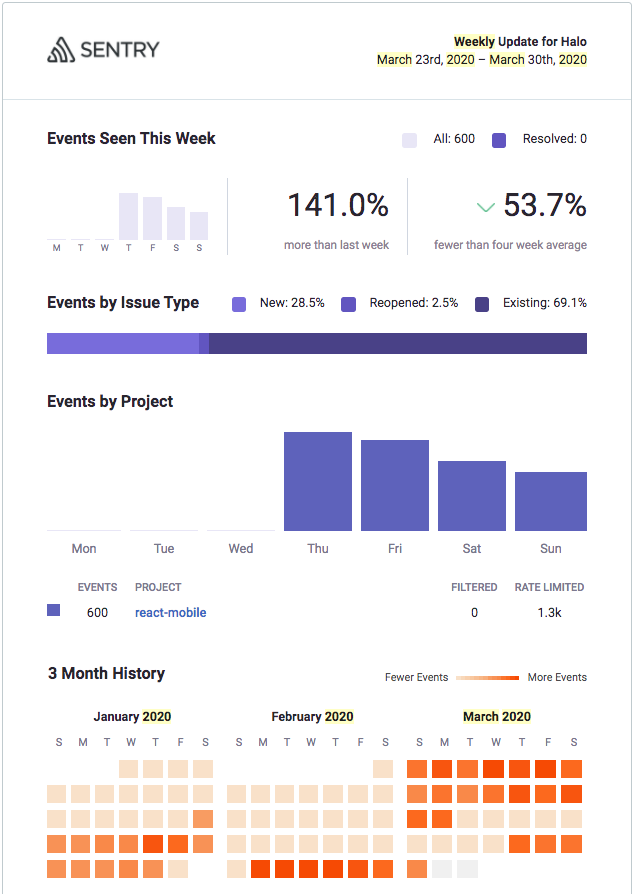
\includegraphics[width=\textwidth]{images/localhalo/sentry-weekly-report-23-mar-2020.png}
  \captionof*{figure}{\nth{23} -~\nth{29} March 2020}
  \label{fig:localhalo-sentry-weekly-report-23-mar-2020}
\end{minipage}
    \caption{Missing data reported in Sentry, in March 2020}
    \label{fig:sentry-missing-data-march-2020}
\end{figure}


\subsection{Developer experience}
After the end of the cases studies, nonetheless of relevance, in June 2022 Google released Canary 3 of the integrated development environment (IDE) called Android Studio Electric Eel. This includes the facility to directly see and work with crashes reported by Firebase Crashlytics within the IDE. This makes the analytics information immediately and continuously available to the developers rather than relying on them visiting the Crashlytics website. It aims to reduce context switching and also encourage faster investigation and remediation of crashes~\citep{android2022_firebase_crash_integration_into_android_studio_electric_eel}.

\section{Fit-for-purpose}


\section{Utility}


\section{Dependability}



\section{Some limits of what can be measured}

Here's a placeholder list, the points will need integrating.
\begin{itemize}
    \item React Native runtime - within runtime crashes vs. application crashes. (LocalHalo and Taskinator apps).
    \item Crashes at startup c.f. private correspondence with Google.
\end{itemize}

\section{Pre-launch reports}
The GTAF project uses pre-launch reports (an intrinsic part of Google Play Console), and the pre-launch report includes automated testing of pre-release apps. The crashes reported in pre-launch reports do not necessarily affect end users. Conversely the pre-launch report automated testing does not find all the failures that affect end users. (Dua \& Zikr app).

Why some projects stopped using pre-launch reports: c.f. the Google bug. TODO add link to the issue on Google and add supporting text.

\section{Flaws in the mobile analytics tools and/or services}

Since 2011, Google has published a list of various changes and corrections to Google Play Console~\citep{google_play_troubleshoot_app_statistics_problems}. During this research numerous additional were discovered that were not published by Google even though their engineering team acknowledged many of these flaws (they chose not to respond to the rest of the flaws). 

\section{Integration and the useful half-life of mobile analytics outputs}
Web-scraping of content from web-sites continues to be a frequent activity performed by many people and services. Web-scraping is used in many fields including bioinfomatics, where the authors discussed why web-scraping was still necessary in a world full of API's~\citet{glez2014_web_scraping_in_an_API_world}. A more recent paper by~\citet{diouf2019_web_scraping_state_of_the_art_and_areas_of_application} briefly presents various inefficiencies in web scraping. Curiously this paper singles out journalism as an under-served area despite it being written about 7 years earlier in Chapter 4 of~\citet{gray2012_the_data_journalism_handbook} (and also covered in a more recent version of the book,~\citet[on pages 133, 238]{bounegru2021_the_data_journalism_handbook}. Suffice to say, web-scraping is a topic that has been written about, albeit not in the context of scraping content from mobile analytics web interfaces. 

API access to mobile analytics has been requested previously~\citep{stackoverflow2013_getting_statistics_from_google_play_developer_console_with_an_api} and various people have developed code that interfaces with Google Play Console in an attempt to provide automated, scripted access to the content.

Our work in developing Vitals Scraper as an opensource project~\citep{vitals_scraper_github_package} and releasing it as an NPM package~\citep{vitals_scraper_npm_package} demonstrates the necessity, viability, and some of the maintenance challenges of writing automated software for web-scraping of outputs from Google Play Console with Android Vitals~\footnote{Note: there was another similar sounding opensource project \url{https://github.com/tmurakam/googleplay_dev_scraper} that provided mechanisms to automate the downloading of the \texttt{csv} monthly reports rather than the live reports. It was last updated in 2013 so no longer current.}. There was also the Andlytics opensource app that provided developers with access to data from their Google Play Console account~\footnote{\url{https://github.com/AndlyticsProject/andlytics}}, however this project also ceased active development for various reasons, probably because Google chose to restrict access to the underlying data in 2019~\footnote{\url{https://github.com/AndlyticsProject/andlytics/issues/766}}. % See also the historic posts by the project on Facebook for screenshots and updates https://www.facebook.com/Andlytics/


None of the mobile analytics tools encountered during the research provided complete access to the outputs using APIs. Furthermore, the ability to record and preserve copies of visual reports (as well as the underlying data) facilitates both practical use of the data in the field (for instance to record the information in an issues tracking database) and for further analysis and research. 

Enterprise-grade mobile analytics services provide mechanisms to export data to homogeneous data storage platforms~\citep{androiddevelopers2015_integrate_play_data_into_your_workflow_with_data_exports}; for instance Google Analytics tools export content to Google Cloud Storage~\footnote{\url{https://support.google.com/googleplay/android-developer/answer/6135870?hl=en-GB}}, and to automate the process~\footnote{\url{https://cloud.google.com/bigquery-transfer/docs/play-transfer}}. Microsoft App Center is unusually complete and provides a comprehensive set of open APIs \url{https://openapi.appcenter.ms/} as well as the ability to export analytics data to Azure \url{https://docs.microsoft.com/en-us/appcenter/analytics/export} and even export data for individual users \url{https://docs.microsoft.com/en-us/appcenter/gdpr/analytics-export}. Google Analytics provides various reporting APIs including those for Exceptions~\footnote{\url{https://ga-dev-tools.web.app/dimensions-metrics-explorer/exceptions}} which are collected by Firebase Analytics for both Android and iOS apps~\footnote{\url{https://developers.google.com/analytics/devguides/collection/firebase/android}}. % See also their github site that underpins the docs https://github.com/googleanalytics/ga-dev-tools

Some of the mobile analytics providers offer developers customisation options such as custom dashboards and reports in Sentry \url{https://docs.sentry.io/product/discover-queries/uncover-trends/}

As a broader observation, various companies provide app analytics services where they obtain the underlying data % See the discussion for https://stackoverflow.com/a/49893656/340175
and aim to provide easy to use, attractive, and actionable reports; examples include \url{https://appfigures.com/} and \url{https://www.data.ai/en/} (previously known as AppAnnie). Appfigures also publishes status reports for the performance of Google Play and Apple's App Store Connect service, these track the publishing performance of these two app stores; at the end of February 2022 they observed Google has been several days late publishing their free daily reports. % Screenshots have been recorded for posterity and are available in my research's appfigures.com folder. 

\section{Differences between mobile analytics tools}
Pocket Code incorporated in-app mobile analytics that recorded both crashes and errors (generally these errors are exceptions that \textit{are} caught and handled by the app) the case study provided the opportunity to study Fabric Crashlytics and to enable its outputs to be compared and contrasted with those from Google Play Console with Android Vitals. \textbf{TODO} discuss the differences.


\section{Improvements to Google Play Console with Android Vitals}

Direct quotes from the CTO of Moodspace (June 2019): \emph{``As for several things I think are missing:''}
\begin{itemize}
    \item \textit{``A gradle plugin to integrate play store uploading into CI processes. I currently use a 3rd party plugin to do this, but it would feel a little more secure if it came from Google.''}
    \item \textit{``Top line core vitals figures even if you don't have enough users!''}
    \item \textit{``Someway for testers to download old apks from either internal app sharing, or the internal release track.''}
\end{itemize}

And \emph{``Crashlytics only covers the crash report of Android vitals, so unfortunately there's no way to get things like battery usage of ANR reports unless Google makes those reports available :(. In terms of crashes, I'd always prefer Crashlytics to Android vitals, simply because there are added features like non-fatal reporting and logs which can make surfacing the cause of errors much easier (but do take need added effort to integrate compared to android vitals).''}

\section{Improving the integration and the useful half-life of mobile analytics outputs}
To discuss, APIs rather than Web Scraping, Persistent and timestamped links to reports (c.f. how github and wikipedia provide versioned links).

In late 2020 Google made various changes to Google Play Console, they provided the ability for developers to directly download individual stacktraces for crashes~\citep{stackoverflow2018_how_can_i_get_app_crash_log_from_google_play_console} which is a useful, small improvement (see \url{https://stackoverflow.com/a/49893656/340175}).


Sentry provides various tools to help development teams focus on key issues,  \url{https://blog.sentry.io/2021/04/20/silencing-distractions-with-review-list-and-automations} (I don't know what information is populated by Sentry when it creates JIRA tickets),  and on the health of new app releases: \url{https://docs.sentry.io/platforms/android/configuration/releases/#release-health}


\section{Discussion on mobile analytics tools and their artefacts}
Mobile Analytics tools need to evolve to remain current and to attract and retain users. Platform tools have a unique advantage compared to in-app tools as the platform tools can collect data across the entire population~\footnote{Subject to opt-outs, sampling, network connectivity, and other reasons the data wouldn't be sent from the overall population.}. For the Android platform, Google Play Console and Android Vitals are able to provide comparisons with apps of peers, both peers selected by app store classifications~\citep{androiddevelopersblog2021_gpc_powers_better_strategic_decisions_etc} and a custom set selected by the developer~\citep{play_console_help_compare_your_apps_android_vitals_and_ratings_with_peer_groups}. 

\section{Summary of tools and their artefacts}
TBC